\documentclass[a4paper,10pt]{article}
\usepackage{tikz}
\usepackage[margin=1in]{geometry}
\usetikzlibrary{automata, positioning, arrows}
\tikzset{->,  % makes the edges directed
>=stealth, % makes the arrow heads bold
node distance=2cm, % specifies the minimum distance between two nodes. Change if necessary.
initial text=$ $, % sets the text that appears on the start arrow
}
\begin{document}
\section{Normal teachers}
\subsection{Normal N requirement (allow first day = N)}
\begin{tabular}{cc}
\begin{tabular}{|c|c|c|c|c|}
\hline
&\tt N&	\tt A&\tt P&\tt O\\
\hline
$1$&$2$&$1$&$1$&$1$\\
\hline
$2$&$0$&$0$&$0$&$1$\\
\hline
\end{tabular}
&
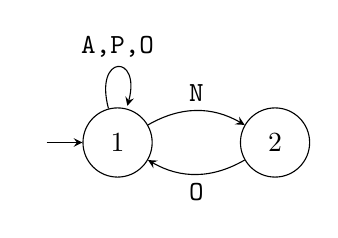
\begin{tikzpicture}
  \node[state, initial] (q1) {$1$};  
  \node[state, right of=q1] (q2) {$2$};
  
  \draw (q1) edge[loop above] node{\tt A,P,O} (q2)
  		(q1) edge[bend left=30, above] node{\tt N} (q2)
		(q2) edge[bend left=30, below] node{\tt O} (q1);

\end{tikzpicture}\\
\end{tabular}
\subsection{At least 1 O for consecutive NW days}
\begin{tabular}{cc}
$NW = 6$\\
\begin{tabular}{|c|c|c|c|c|}
\hline
&\tt N&\tt A&\tt P&\tt O\\
\hline
$1$&$2$&$2$&$2$&$1$\\
\hline
$2$&$3$&$3$&$3$&$1$\\
\hline
$3$&$4$&$4$&$4$&$1$\\
\hline
$4$&$5$&$5$&$5$&$1$\\
\hline
$5$&$6$&$6$&$6$&$1$\\
\hline
$6$&$0$&$0$&$0$&$1$\\
\hline
\end{tabular}
&
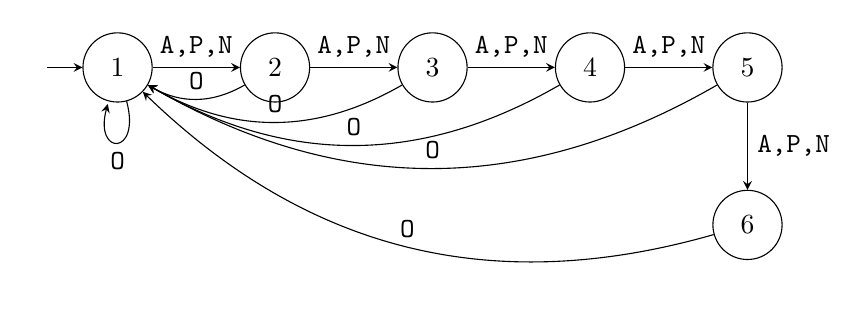
\begin{tikzpicture}
  \node[state, initial] (q1) {$1$};
  \node[state, right of=q1] (q2) {$2$};
  \node[state, right of=q2] (q3) {$3$};
  \node[state, right of=q3] (q4) {$4$};
  \node[state, right of=q4] (q5) {$5$};
  \node[state, below of=q5] (q6) {$6$};
  
  \draw (q1) edge[loop below] node{\tt O} (q1)
  		(q1) edge[above] node{\tt A,P,N} (q2)
  		(q2) edge[above] node{\tt A,P,N} (q3)
  		(q3) edge[above] node{\tt A,P,N} (q4)
  		(q4) edge[above] node{\tt A,P,N} (q5)
  		(q5) edge[right] node{\tt A,P,N} (q6)
  		(q2) edge[bend left, above] node{\tt O} (q1)
  		(q3) edge[bend left, above] node{\tt O} (q1)
  		(q4) edge[bend left, above] node{\tt O} (q1)
  		(q5) edge[bend left, above] node{\tt O} (q1)
  		(q6) edge[bend left, above] node{\tt O} (q1);

\end{tikzpicture}\\
\end{tabular}
\section{Night teachers}
\subsection{At least 2 Os for consecutive 4 Ns}
\begin{tabular}{cc}
\begin{tabular}{|c|c|c|c|c|}
\hline
&\tt N&\tt A&\tt P&\tt O\\
\hline
$1$&$2$&$0$&$0$&$1$\\
\hline
$2$&$3$&$0$&$0$&$1$\\
\hline
$3$&$4$&$0$&$0$&$1$\\
\hline
$4$&$5$&$0$&$0$&$1$\\
\hline
$5$&$0$&$0$&$0$&$6$\\
\hline
$6$&$0$&$0$&$0$&$1$\\
\hline
\end{tabular}
&
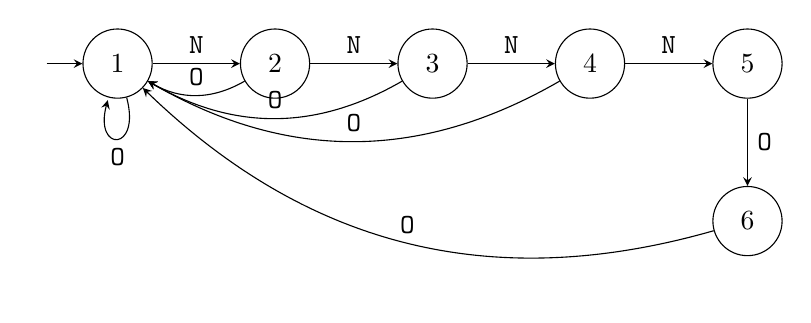
\begin{tikzpicture}
  \node[state, initial] (q1) {$1$};
  \node[state, right of=q1] (q2) {$2$};
  \node[state, right of=q2] (q3) {$3$};
  \node[state, right of=q3] (q4) {$4$};
  \node[state, right of=q4] (q5) {$5$};
  \node[state, below of=q5] (q6) {$6$};
  
  \draw (q1) edge[loop below] node{\tt O} (q1)
  		(q1) edge[above] node{\tt N} (q2)
  		(q2) edge[above] node{\tt N} (q3)
  		(q3) edge[above] node{\tt N} (q4)
  		(q4) edge[above] node{\tt N} (q5)
  		(q5) edge[right] node{\tt O} (q6)
  		(q2) edge[bend left, above] node{\tt O} (q1)
  		(q3) edge[bend left, above] node{\tt O} (q1)
  		(q4) edge[bend left, above] node{\tt O} (q1)
  		(q6) edge[bend left, above] node{\tt O} (q1);

\end{tikzpicture}\\
\end{tabular}
\end{document}